\documentclass[cn,chinese,founder]{elegantbook}
\usepackage{wrapfig}
\everymath{\displaystyle}

\begin{document}
    \chapter{章节名}
        \section{节名}
            \subsection{思考题}
            \begin{example}
                思考题一
                \begin{enumerate}
                    \item 第(1)小问
                    \begin{enumerate}
                        \item 第(i)小问
                    \end{enumerate}
                    \item 第(2)小问
                \end{enumerate}
            \end{example}
            \begin{wrapfigure}{r}{3.5cm}
                \vspace{-1.5cm}
                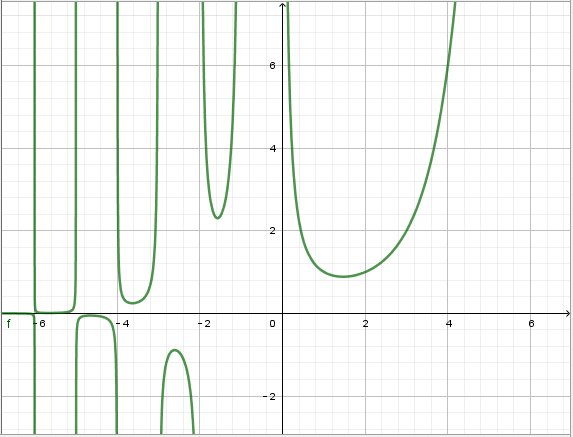
\includegraphics[width=3.5cm]{example.png}
                \caption[示例]{示例解答图片}
            \end{wrapfigure}
            \begin{solution}
                解答
            \end{solution}
            
            \subsection{练习题}
            \begin{exercise}
                练习题一
            \end{exercise}
            \begin{solution}
                解答
            \end{solution}
\end{document}